\documentclass[12pt]{article}

\usepackage{hyperref}
\hypersetup{
    colorlinks=true,
    linkcolor=blue,
    filecolor=blue,      
    urlcolor=blue,
    pdftitle={Bayesian Analysis Project},
    pdfpagemode=FullScreen,
    }

\usepackage[utf8]{inputenc}
\usepackage[T1]{fontenc}
\usepackage{subfig}
\usepackage[backend=biber, style=apa, sorting=ynt]{biblatex}
\setlength\bibitemsep{1.9\itemsep}
\addbibresource{ref.bib}
\usepackage{float}
\usepackage[a4paper,top=2.5cm,bottom=2cm,left=2cm,right=2cm,marginparwidth=1.75cm]{geometry}
\usepackage{amssymb,amsmath,amsthm,enumitem}
\usepackage{graphicx}
\usepackage{array}
\usepackage{multirow}
\setlength{\parskip}{1em}
\setlength{\parindent}{0em}
\setlength{\intextsep}{10pt plus 2pt minus 2pt}

\begin{document}

\begin{titlepage}

\newcommand{\HRule}{\rule{\linewidth}{0.5mm}}
\center 
 
\textsc{\LARGE Universitá degli studi di Milano}\\[1cm]

\bigskip

\textsc{\Large Bayesian Analisis}\\[0.2cm]
\textsc{\Large M.Sc. Data Science \& Economics}\\[0.2cm]

\bigskip
\bigskip
\bigskip
\HRule \\[0.8cm]
\bigskip

{ \huge \bfseries Which factors are contributing to Greenhouse gas emissions in Italy?}\\[0.7cm]
\HRule \\[2cm]
\large
\emph{David A. Heilbron}  \ \ \ \emph{Alessia Leo Folliero} \\
Code: 988346 \ \ \ Code: 08399A\\[1.5cm]
{\large \today}\\[5cm]
\includegraphics[width=0.6\textwidth]{images/Intro/Logo.jpg}\\[1cm]
\vfill 
\end{titlepage}


\tableofcontents
\clearpage


\section{Introduction}

In this project we are going to analyze a time series from 1990 to 2020 of net greenhouse gas emissions per capita (yearly data) for Italy. Our objective is to understand which are the most relevant factors that contribute to the increase (or decrease) of the total amount of greenhouse gasses produced every year. 

The emission of greenhouse gasses is closely related to climate change and it leads to many consequences to our environment such as the increase in temperature, increased frequency of severe storms, increases in droughts, a warming rising ocean and many other \footnote{ \emph{The consequences of the greenhouse effect: from desertification to floods} \url{https://bit.ly/40QZcjq}}. 

To help fight climate change the EU has set targets to reduce its greenhouse gas emissions, with the aim to reach climate neutrality by 2050. This target gets along with an interim target of 40\%\ greenhouse gasses emission reduction by 2030. The proposed national target to Italy (to be reached in 2030) is a reduction of 43.7\%\ of greenhouse gases emissions with respect to 2005 \footnote{ \emph{Cutting EU greenhouse gas emissions: national targets for 2030} \url{https://bit.ly/3Nw8EFL}}. 

But what are greenhouse gasses and how are they composed? 

Definition from Britannica\footnote{See \url{https://bit.ly/3Nrgbpv}}:  \emph{"any gas that has the property of absorbing infrared radiation (net heat energy) emitted from Earth’s surface and reradiating it back to Earth’s surface, thus contributing to the greenhouse effect. Carbon dioxide, methane, and water vapour are the most important greenhouse gases"}. As seen in Figure \ref{fig:Fig1}, around 90\%\ of the greenhouse gas emissions come from carbon dioxide and methane \footnote{ \emph{Greenhouse gas emissions} \url{https://bit.ly/423jXKk}}. \\

 \begin{figure}[H]
    \centering
    \includegraphics[width=0.8\textwidth]{images/Intro/Intro_1.png}
    \caption{Greenhouse gases composition}
    \label{fig:Fig1}
\end{figure}

Moreover, as depicted in Figure \ref{fig:Fig2} the main sectors that do contribute to production of greenhouse gas are transport, agriculture, buildings, waste management and deforestation \footnote{ \emph{Sector by sector: where do global greenhouse gas emissions come from?} \url{https://bit.ly/42hpkoJ}}.

 \begin{figure}[H]
    \centering
    \includegraphics[width=0.8\textwidth]{images/Intro/Intro_2.png}
    \caption{Greenhouse gas emissions by sector}
    \label{fig:Fig2}
\end{figure}

Having this in mind, the analysis that follows is focused on estimating three different Vector Autoregressive (VAR) models including factors that are related to greenhouse gas emissions. Estimation will be done using a Bayesian approach, to later forecast their Impulse Response Functions (IRF). We are interested in the response of net greenhouse gases emissions per capita to a shock coming from the other variables in the models. 

The rest of the paper is structured as follows: Section \ref{Dataset} discusses data and its processing before estimating the models; Section \ref{Bayesian VAR Models} discusses the VAR models, priors, posteriors and the Markov Chain Monte Carlo (MCMC) algorithms used to estimate coefficients; Section \ref{Models & Results} shows estimation results and the forecasted IRFs; and Section \ref{Conclusions} estates the conclusions of the analysis and suggestions for future improvement.

\clearpage

\section{Dataset} \label{Dataset}
After doing some research about the main factors that could contribute positively or negatively to the emissions of greenhouse gases, several different variables were included in the dataset. They range from 1990 to 2020 and are measured yearly, covering only Italy. Our variable of interest is net greenhouse gasses which is measured in tonne per capita of greenhouse gasses emissions. A summary of the variables and their unit of measure is shown in \ref{tab:variables}. \\

\begin{table}[H]
    \begin{center}
    \begin{tabular}{ll} \hline
    \multicolumn{1}{c}{\textbf{Features}} & \multicolumn{1}{c}{\textbf{Unit of measure}} \\ \hline
        Net greenhouse gas emissions  & tonnes per capita \\
        Environmental taxes  & percentage of GDP \\
        GDP pc & Constant 2010 US dollars \\
        Industrial production  & Index 2015=100 \\
        Energy imp dep & percentage \\
        Naturalgas imports & Million $m^3$ \\
        Oil imports & Thousand tonnes \\
        Total energy supply & Gigawatt-hour \\ 
        Gross electricity production & Gigawatt-hour \\
        Share of land under permanent crops & percntage \\
        Area harvested Rice & Area ha \\
        Fertilizer used per area of cropland & kg per ha \\
        Share in land area Forest Land & percentage \\ 
        Rail tracks KM & km \\
        Length of motorways & km \\
        Number of motorcycle & Units \\
        Total freight loaded and unloaded & tonnes \\
        Livestock heads & Thousand heads \\
        RES capacity & Megawatt \\ \hline
    \end{tabular}
    \caption{Variables description} \label{tab:variables}
    \end{center}
\end{table}

The variable $livestock\_heads$ includes the following type of livestock: pigs, sheeps, goats, chicken, turkey, cattle and buffalos. Measured in thousand heads. On the other hand, the variable $res\_capacity$, which is short for 'renewable energy source', measures the installed capacity of renewable energy at a given year, and includes the following sources: hydro, geothermal, wind, solar, biofuels, biogas and waste. \\

\clearpage
\subsection{Data pre-processing} \label{Data pre-processing}
After the upload of the dataset in Rstudio some preprocessing steps were needed.\\

The first step was characterized by variable encoding and the imputation of some missing values in the variables: Rail tracks KM, Total freight loaded and unloaded, Chicken heads and Turkeys heads.
The imputation of data was done using the “Spline” method which from literature is preferred to polynomial interpolation and avoid also the Runge’s phenomenon.\\
The next step was represented by the visual analysis of the distribution of the features: \\

 \begin{figure}[H]
    \centering
    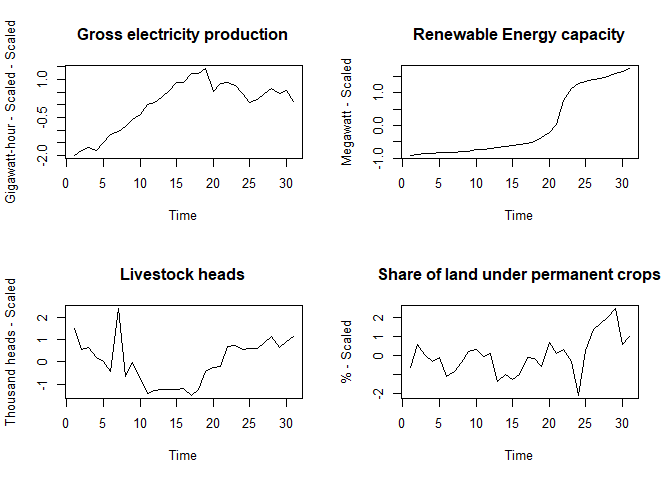
\includegraphics[width=0.8\textwidth]{images/Preprocessing/5-1.png}
    \caption{Net greenhouse gasses emissions, Environmental taxes, GDP per capita and Industrial production}
    \label{fig:Fig3}
\end{figure}
\begin{figure}[H]
    \centering
    \includegraphics[width=0.8\textwidth]{images/Preprocessing/5-2.png}
    \caption{Energy imports dependency, Natural gas imports, Oil imports and Total energy supply}
    \label{fig:Fig4}
\end{figure}
\begin{figure}[H]
    \centering
    \includegraphics[width=0.8\textwidth]{images/Preprocessing/5-3.png}
    \caption{Gross electricity production, Renewable Energy capacity, Livestock heads and Share of land under permanent crops}
    \label{fig:Fig5}
\end{figure}
\begin{figure}[H]
    \centering
    \includegraphics[width=0.8\textwidth]{images/Preprocessing/5-4.png}
    \caption{Harvested rice, Fertilizers used per ha of cropland,Share of forest land and Rail tracks}
    \label{fig:Fig6}
\end{figure}
\begin{figure}[H]
    \centering
    \includegraphics[width=0.8\textwidth]{images/Preprocessing/5-5.png}
    \caption{Length of motorways, Number of motorcycles and Total aerial freight}
    \label{fig:Fig7}
\end{figure}


Then since all the variables are explained in different measure units, variables were scaled and furthermore we took the first difference of all them.


\section{Bayesian VAR Models \& Gibbs sampler} \label{Bayesian VAR Models}

As shown in (\cite{canova2013panel}), a Vector Autoregressive model of lag \emph{p} can be characterized by Equation \ref{VAR_model_1}. Let $Y_{t}$ be a \emph{N} x 1 vector of endogenous variables; $A_{0}$ the \emph{N} x 1 vector of intercepts and $A_{i}$ for $i = 1, ..., p$ the \emph{N} x \emph{N} matrix of coefficients. The VAR(p) for $Y_{t}$ is:

\begin{equation}\label{VAR_model_1}
Y_{t} = A_{0} + A_{1}Y_{t-1} + ... + A_{p}Y_{t-p} + e_{t}  \quad e_{t} \sim N(0, \Sigma)
\end{equation}

Where $A_{l}$ is a polynomial in the lag operator and errors are \emph{iid}, identically and independently distributed.  We are interested in estimating $A_{0}$, $A_{1}, ..., A_{p}$ and $\Sigma$, which is the \emph{N} x \emph{N} variance-covariance matrix of the error. The model can be represented in its vector form as: 

\begin{equation}\label{VAR_model_2}
Y_{t} = X_{t}\beta + e_{t} \\[1pt]
\end{equation}

Where $\beta = vec([A_{0}, A_{1}, ..., A_{p}]')$ and $X_{t} = (I_{n} \otimes [1, y_{t-1}^{'}, ..., y_{t-p}^{'}])$. The model can be stacked over time t to obtain the compact form:

\begin{equation}\label{VAR_model_3}
Y = X\beta + E \\[1pt] \quad \text{where} \quad E \sim N(0, I_{T} \otimes \Sigma)
\end{equation}

Where $Y$ and $E$ are \emph{T} x \emph{N} matrices and $X$ is a \emph{T} x (\emph{N}x\emph{p}) matrix. As it can be seen, the model in Equation \ref{VAR_model_3} is a multivariate regression representation of equation \ref{VAR_model_1}. For this model, a likelihood function could be provided in the form of

\begin{equation}\label{Likelihood_1}
\mathcal{L}(y | \beta, \Sigma) = |2\pi (I_{T} \otimes \Sigma)|^{-0.5} exp\{-0.5(y-X\beta)^{'}(I_{T} \otimes \Sigma^{-1})(y-X\beta)\}
\end{equation}

Following (\cite{canova2007methods}) and omitting some steps for simplicity, it can be shown that the Likelihood function of a VAR(p) model can be there decomposed into the product of a Normal density for $\beta$ and a Wishart density for $\Sigma^{-1}$ in the following form

\begin{equation}\label{Likelihood_2}
\mathcal{L}(y | \beta, \Sigma) \propto \mathbb{N} (\beta | \beta_{ols}, \Sigma, X, Y)\  \text{x} \ \mathbb{W} (\Sigma^{-1} | Y, X, \beta_{ols}, df)
\end{equation}

Where $\beta_{ols}$ is the OLS estimation for the vector of coefficients and \emph{df} are the \emph{T}$-$\emph{k}$-$\emph{n}$-$1 degrees of freedom of the Wishart distribution.

\subsection{Priors and Conditional Posterior distributions}

To estimate the full conditional posterior distributions of $\beta$ and $\Sigma^{-1}$ we follow (\cite{canova2007methods}) once again, who shows that a Normal-Wishart prior conjugates the two blocks of the likelihood function, hence the resulting conditional posterior  for $\beta$ is a Normal distribution and the conditional posterior for $\Sigma^{-1}$ is a Wishart distribution. Equations \ref{Posterior_beta} describes the conditional posterior for the coefficients of the VAR(p) model.

\begin{equation}\label{Posterior_beta}
\begin{split}
\pi(\beta | \Sigma, y) \propto exp\{-0.5(y-X\beta)^{'}(I_{T} \otimes \Sigma^{-1})(y-X\beta)\} \\ \cdot exp\{-0.5(\beta-\mu_{\beta})^{'}V_{\beta}^{-1}(\beta-\mu_{\beta})\} \ \sim N(A, B)
\end{split}
\end{equation}

where \emph{B} = $V_{\beta}^{-1}$ + $X^{'}(I_{T} \otimes \Sigma^{-1})X$, and \emph{A} = $B^{-1}(V_{\beta}^{-1}\beta_{0}+X^{'}(I_{T} \otimes \Sigma^{-1})y)$, $\mu_{\beta}$ is the mean over $\beta$ and $V_{\beta}$ the variance. For $\Sigma^{-1}$ the conditional posterior density is described as follows.

\begin{equation}\label{Posterior_Sigma}
\begin{split}
\pi(\Sigma | \beta, y) \propto |\Sigma| ^{\frac{-\nu_{0}+T+n+1}{2}} \cdot exp\{-0.5 \cdot tr(S_{0}\Sigma^{-1}\}   \\
\cdot exp\{-0.5 \cdot tr(\sum^{T}_{t=1} (y_{t}-X_{t}\beta)^{'}(y_{t}-X_{t}\beta)\Sigma^{-1})\} \\
\sim iW(\nu_{0}+T, S_{0}+\Sigma(y_{t}-X_{t}\beta)(y_{t}-X_{t}\beta)^{'})
\end{split}
\end{equation}

Where \emph{iW} denotes an inverse Wishart distribution, tr($\cdot$) is the trace of a matrix, $\nu_{0}$+\emph{T} are the degrees of freedom and  $S_{0}+\Sigma(y_{t}-X_{t}\beta)(y_{t}-X_{t}\beta)^{'}$ is the scale of the distribution.

\subsection{Generalized Impulse Response Function}

Our analysis of the different factors affecting the net greenhouse gases emissions will be carried on by computing the Generalized Impulse Response Function (GIRF) of our different VAR models. Like stated in (\cite{pesaran1998generalized}), the GIRF avoids the shortcomming of the ordering of the variables while providing consistent and asymptotically normally distributed coefficients.

The GIRF is calculated from the moving average representation of a VAR model, as the difference between a conditional and unconditional forecast, where the conditioning information set is the schock to the $j_{th}$ variable (\cite{koop1996impulse}). Considering the following recursive moving average representation of a VAR(p) model, where $A_{i}$ is the \emph{m}x\emph{m} coefficient matrix

\begin{equation}\label{GIRF_1}
\begin{split}
A_{i} = \Phi_{1}A_{i-1}+\Phi_{2}A_{i-2}+\cdot \cdot \cdot + \Phi_{p}A_{i-p} \quad i=1, 2, ..., p
\end{split}
\end{equation}

With $A_{0}=I_{m}$ and $A_{i}=0$ for $i<0$, and $G_{i}=A_{i}\Phi$, where $G_{i}$ is the \emph{q}x\emph{q} matrix of coefficients of the deterministic and/or exogenous variables. Denoting the known history of the time series up to time $t-1$ by the non-decreasing information set $\Omega_{t-1}$, and the vector of scocks $\delta=(\delta_{1},...,\delta_{m})^{'}$, the GIRF of $x_{t}$, where $x_{t}=(x_{1t}, x_{2t},...,x_{mt})^{'}$ is an $m$x1 vector of dependent variables, at horizon $n$ is defined by

\begin{equation}\label{GIRF_2}
\begin{split}
GI_{x}(n,\delta,\Omega_{t-1)}) = E(x_{t+n}|\varepsilon_{t}=\delta, \Omega_{t-1})-E(x_{t+n}|\Omega_{t-1})
\end{split}
\end{equation}

Although it is not the scope of this paper, it can be demonstrated that Equation\ref{GIRF_2} can be scaled and represented in the following form

\begin{equation}\label{GIRF_2}
\begin{split}
\psi_{j}^{g}(n) = \sigma_{jj}^{-\frac{1}{2}}A_{n}\Sigma e_{j} \quad n=0,1,2,...
\end{split}
\end{equation}

which measures the effect of one standard error shock to the $j_{th}$ equation at time $t$ on expected values of $x$ at time $t+n$. From the above representation it can be derived the forecast error variance  decomposition (FEVD), defined as the proportion of the $n$-step ahead forecast error variance  of variable $i$ which is accounted for by the innovations in variable $j$ in the VAR(p) (\cite{pesaran1998generalized}). For $n=0,1,2,...$, the generalized FEVD is represented by

\begin{equation}\label{GIRF_2}
\begin{split}
\theta_{ij}^{g}(n)=\frac{\sigma_{ii}^{-1}\Sigma_{l=0}^{n}(e_{i}^{'}A_{l}\Sigma e_{j})^{2}}{\Sigma_{l=0}^{n}e^{'}_{i}A_{l}\Sigma A_{l}^{'}e_{i}} \quad i,j=1,...,m
\end{split}
\end{equation}


\subsection{Gibss sampler}

To approximate the full conditional posterior distributions obtained in Section \ref{Bayesian VAR Models}, a Markov-Chain Monte-Carlo (MCMC) algorithm will be used, specifically Gibbs sampler . As we did arrive to a closed-form  posterior densities for $\beta$ and $\Sigma$, Gibbs sampler would be a proper algorithm to approximate our posterior distributions (\cite{hoff2009first}). 

Recall that for two given posterior distributions of $\theta$ and $\sigma^{2}$, i.e., $p(\theta|\sigma^{2},y_{1},...,y_{n})$ and $p(\sigma^{2}|\theta, y_{1},...,y_{n})$, given an initial state of parameters $\phi^{(s)}=\{\theta^{(s)}, \tilde{\sigma}^{(s)}\}$ a new state can generated as follows

\begin{enumerate}
  \item sample $\theta^{(s+1)} \sim p(\theta|\tilde{\sigma}^{2},y_{1},...,y_{n})$ ;
  \item sample $\tilde{\sigma}^{2(s+1)} \sim p(\tilde{\sigma}^{2}|\theta^{(s+1)}, y_{1},...,y_{n})$ ;
  \item let $\phi^{(s+1)} =\{\theta^{(s+1)}, \tilde{\sigma}^{(s+1)}\}$
\end{enumerate}

The Gibbs sampler then generates a dependent sequence of parameters $\{\phi^{(1)} , \phi^{(2)} ,...,\phi^{(S)}\}$ where $S$ denotes the number of iterations of the algorithm. For our specific application, our full conditional densities over $\beta$ and $\Sigma$ are described as

\begin{equation}
\begin{split}
   \{\beta|y_{1},...,y_{n},\Sigma\}\sim \text{multivariate normal}(\mu_{n},\Lambda_{n}) \\
   \{\Sigma|y_{1},...,y_{n},\beta\}\sim \text{inverse-Wishart}(\nu_{n},S^{-1}_{n})
   \end{split}
\end{equation}

Given a stating value $\Sigma^{0}$, the Gibbs sampler generates $\{\beta^{(s+1)},\Sigma^{(s+1)}\}$ from $\{\beta^{(s)},\Sigma^{(s)}\}$ as follows

\begin{enumerate}
  \item sample $\beta^{(s+1)}$ from its full conditional density:
  \begin{enumerate}
      \item compute $A$ and $B$ from $y_{1},...,y_{n}$ and $\Sigma^{(0)}$ using OLS;
      \item sample $\beta^{(s+1)} \sim \text{multivariate normal}(A,B)$.
  \end{enumerate}
  \item sample ${\Sigma}^{(s+1)}$ from its full conditional distribution:
  \begin{enumerate}
      \item compute $S_{n}$ from $y_{1},...,y_{T}$ and $\beta^{(s+1)}$;
      \item sample ${\Sigma}^{(s+1)} \sim \text{inverse-Wishart}(\nu_{0}+T, S_{0}+\Sigma(y_{t}-X_{t}\beta^{(s+1)})(y_{t}-X_{t}\beta^{(s+1)})^{'})$
  \end{enumerate}
  
\end{enumerate}

where $A=B^{-1}(V_{\beta}^{-1}\beta_{0}+X^{'}(I_{T}\otimes \Sigma^{-1})y)$ and $B+V_{\beta}^{-1}+X^{'}(I_{T}\otimes \Sigma^{-1})X$ as obtained in Section \ref{Bayesian VAR Models}. Our prior beliefs on the parameters which will start the Gibbs sampler are

\begin{enumerate}
    \item $\beta_{0} = \beta_{OLS}$
    \item $V_{\beta}^{-1} = I_{T}$
    \item $\Sigma^{-1} = \Sigma^{-1}_{OLS}$
    \item $\nu_{0}=2*n$
    \item $S_{0} = T_{T}$
\end{enumerate}

The sampler was run for $S=20,000$ iterations with a burn-in of 2,000, no thinning was performed as the ACF plots of the coefficients didn't suggest any autocorrelation. Although not displayed here for simplicity, output analysis and convergence analysis were carried on, suggesting convergence of the chains and an even lower number of iterations and burn-in needed to achieve it. The chains, ACF plots and densities can be seen in the Appendix.

\clearpage

\section{Models \& Results} \label{Models & Results}

In this section we present three different models taken from the original dataset. Although we tested several features and combinations, these were the ones that show a considerable response to our research question. The number of lags $p$ were selected using the Schwarz Information criterion, which for each of the three models suggested number of lags to be $p=1$. The models are then described as the following VAR(1) representation

\begin{equation}\label{GIRF_2}
\begin{split}
y^{1}_{t} = \alpha_{0}^{1}+\alpha_{11}y^{1}_{t-1}+\alpha_{12}y^{2}_{t-1}+\alpha_{13}y^{3}_{t-1}+\varepsilon^{1}_{t} \\
y^{2}_{t} = \alpha_{0}^{2}+\alpha_{21}y^{1}_{t-1}+\alpha_{22}y^{2}_{t-1}+\alpha_{23}y^{3}_{t-1}+\varepsilon^{2}_{t} \\
y^{3}_{t} =\alpha_{0}^{3}+ \alpha_{31}y^{1}_{t-1}+\alpha_{32}y^{2}_{t-1}+\alpha_{33}y^{3}_{t-1}+\varepsilon^{3}_{t} \\
\end{split}
\end{equation}

where $\varepsilon^{m}_{t}$ $\sim N(0,\Sigma)$ for $m=(1,2,3)$. In Table \ref{tab:models_spec} the different variables used in each model are specified.

\begin{table}[H]
    \begin{center}
     \begin{tabular}{llll} \hline
         & \multicolumn{1}{c}{\textbf{$y^{1}_{t}$}}  & \multicolumn{1}{c}{\textbf{$y^{2}_{t}$}} & \multicolumn{1}{c}{\textbf{$y^{3}_{t}$}} \\ \hline
        Model 1 & Greenhouse gas & Harvested rice & Permanent crops \\
        Model 2 & Greenhouse gas & Energy imports dependency & Oil imports \\
        Model 3 & Greenhouse gas & GDP per capita & Fertilizer \\ \hline
    \end{tabular}
    \end{center}
    \caption{Variables per model} \label{tab:models_spec}
\end{table}

In what follows, the estimated vectors of coefficients from the Gibss sampler are displayed and compared against the OLS estimation. 

\subsection*{Model 1} \label{Results_model1}

As it can be seen in Table \ref{tab:tab_beta_1}, the estimated coefficients are virtually equal in the OLS and Bayesian estimation. Regarding the variance-covariance matrix provided in Table \ref{tab:tab_sigma_1} the Bayesian estimates provide a slightly lesser variability than the OLS estimates for the variance of $crops_{t-1}$ and $rice_{t-1}$ while for $greenhouse_{t-1}$ the variance is lesser in the OLS estimate.\\

\begin{table}[H]
\centering
\begin{tabular}{|l|c|c|c|c|c|c|c|c|}
  \hline
 \multirow{2}{*}{Model 1 $\hat{\beta}$} & \multicolumn{2}{c|}{$greenhouse_{t-1}$} & \multicolumn{2}{c|}{$rice_{t-1}$}  & \multicolumn{2}{c|}{$crops_{t-1}$} & \multicolumn{2}{c|}{$const$} \\  \cline{2-9}
 & $\hat{\beta}_{ols}$ & $\hat{\beta}_{B}$ & $\hat{\beta}_{ols}$ & $\hat{\beta}_{B}$ & $\hat{\beta}_{ols}$ & $\hat{\beta}_{B}$ & $\hat{\beta}_{ols}$ & $\hat{\beta}_{B}$\\
  \hline
    $greenhouse_{t}$ & 0.14 & 0.14 & 0.08 & 0.08 & 0.14  &  0.14 &  -0.08  & -0.08  \\ 
    $rice_{t}$ & -0.99 & -0.99 & 0.21 &  0.21 & 0.04 & 0.04 &-0.01 & -0.01\\ 
    $crops_{t}$ & -0.38 & -0.38 & 0.03 & 0.02 & -0.20 & -0.20 & -0.01 & -0.01 \\ 
   \hline
\end{tabular}
\caption{Bayesian and OLS estimation of $\hat{\beta}$, Model 1} \label{tab:tab_beta_1}
\end{table}

\begin{table}[H]
\centering
\begin{tabular}{|l|c|c|c|c|c|c|c|c|}
  \hline
 \multirow{2}{*}{Model 1 $\hat{\Sigma}$}& \multicolumn{2}{c|}{$greenhouse_{t-1}$} & \multicolumn{2}{c|}{$rice_{t-1}$}  & \multicolumn{2}{c|}{$crops_{t-1}$} \\  \cline{2-7}
 & $\hat{\Sigma}_{ols}$ & $\hat{\Sigma}_{B}$ & $\hat{\Sigma}_{ols}$ & $\hat{\Sigma}_{B}$ & $\hat{\Sigma}_{ols}$ & $\hat{\Sigma}_{B}$ \\
  \hline
    $greenhouse_{t-1}$ & 0.07 & 0.11 & 0.03 & 0.02 & 0.00  &  0.00   \\ 
    $rice_{t-1}$ & 0.03 & 0.02 & 0.71 &  0.69 & 0.12 & 0.11 \\ 
    $crops_{t-1}$ & 0.00 & 0.00 & 0.12 & 0.11 & 0.82 & 0.79 \\ 
   \hline
\end{tabular}
\caption{Bayesian and OLS estimation of $\hat{\Sigma}$, Model 1} \label{tab:tab_sigma_1}
\end{table}

Next comes the forecasted generalized impulse responses. Figure \ref{fig:IRF1_1} depicts the response of net greenhouse gases emissions per capita to a one standard deviation increase in hectares of harvested rice. On the other hand, Figure \ref{fig:IRF1_2} displays the response of net greenhouse gases emissions per capita to a one standard deviation shock of share of land under permanent crops.The behavior of the response variable to these shocks may confirm the fact that the current methods for agriculture may be contributing to the accumulation of greenhouse gases in the atmosphere.\\

 \begin{figure}[H]
    \centering
    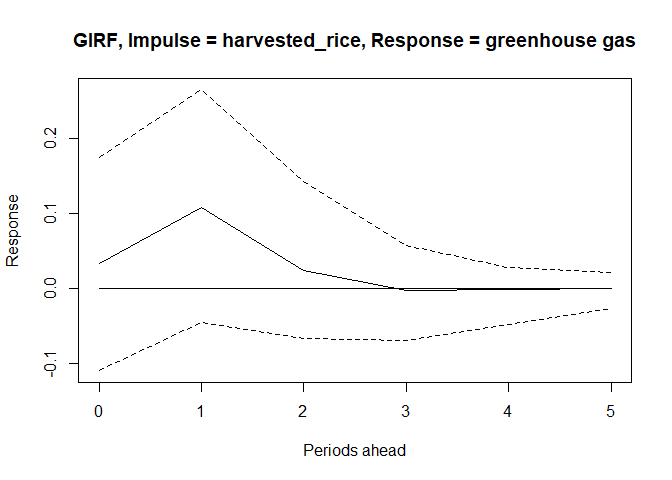
\includegraphics[width=0.7\textwidth]{images/IRF/IRF Analysis model 1-1.png}
    \caption{Forecasted impulse response}
    \label{fig:IRF1_1}
\end{figure}

 \begin{figure}[H]
    \centering
    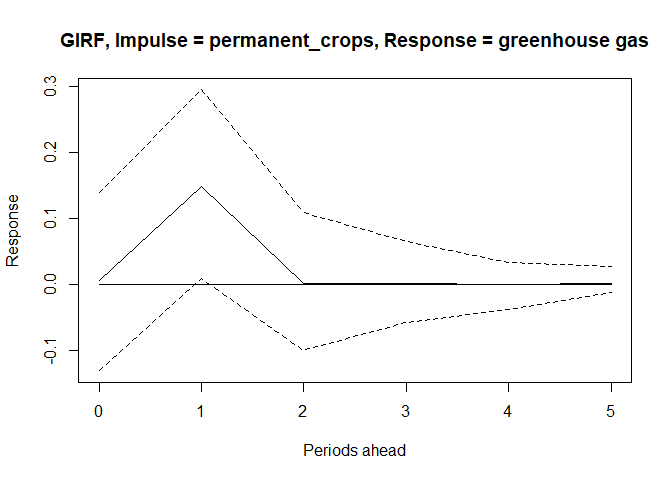
\includegraphics[width=0.7\textwidth]{images/IRF/IRF Analysis model 1-2.png}
    \caption{Forecasted impulse response}
    \label{fig:IRF1_2}
\end{figure}

%\clearpage

\subsection*{Model 2} \label{Results_model2}

Table \ref{tab:tab_beta_2} shows again the coefficients for both the frequentist and the bayesian estimation methods. Regarding the variance-covariance matrix provided in Table \ref{tab:tab_sigma_2} the variance of $greenhouse_{t-1}$ and $oil\_imports_{t-1}$ is higher for the Bayesian estimate, while the covariances are slightly lower. \\

\begin{table}[H]
\centering
\label{tab:tab_beta_2}
\begin{tabular}{|l|c|c|c|c|c|c|c|c|}
  \hline
 \multirow{2}{*}{Model 2 $\hat{\beta}$} & \multicolumn{2}{c|}{$greenhouse_{t-1}$} & \multicolumn{2}{c|}{$energy\_dep_{t-1}$}  & \multicolumn{2}{c|}{$oil\_imports_{1}$} & \multicolumn{2}{c|}{$const$} \\  \cline{2-9}
 & $\hat{\beta}_{ols}$ & $\hat{\beta}_{B}$ & $\hat{\beta}_{ols}$ & $\hat{\beta}_{B}$ & $\hat{\beta}_{ols}$ & $\hat{\beta}_{B}$ & $\hat{\beta}_{ols}$ & $\hat{\beta}_{B}$\\
  \hline
    $greenhouse_{t}$ & -0.06 & -0.06 & 0.12 & 0.12 & 0.19  &  0.20 &  -0.07  & -0.07  \\ 
    $energy\_dep_{t}$ & 0.14 & 0.14 & -0.51 &  -0.51 & -0.02 & -0.02 &-0.12 & -0.12\\ 
    $oil\_imports_{t}$ & 0.01 & 0.01 & -0.02 & -0.02 & -0.04 & -0.04 & -0.10 & -0.10 \\ 
   \hline
\end{tabular}
\caption{Bayesian and OLS estimation of $\hat{\beta}$, Model 2} \label{tab:tab_beta_2}
\end{table}

\begin{table}[H]
\centering
\begin{tabular}{|l|c|c|c|c|c|c|c|c|}
  \hline
 \multirow{2}{*}{Model 2 $\hat{\Sigma}$} & \multicolumn{2}{c|}{$greenhouse_{t-1}$} & \multicolumn{2}{c|}{$energy\_dep_{t-1}$}  & \multicolumn{2}{c|}{$oil\_imports_{1}$} \\  \cline{2-7}
 & $\hat{\Sigma}_{ols}$ & $\hat{\Sigma}_{B}$ & $\hat{\Sigma}_{ols}$ & $\hat{\Sigma}_{B}$ & $\hat{\Sigma}_{ols}$ & $\hat{\Sigma}_{B}$ \\
  \hline
    $greenhouse_{t-1}$ & 0.09 & 0.12 & 0.09 & 0.08 & 0.09  &  0.08   \\ 
    $energy\_dep_{t-1}$ & 0.09 & 0.08 & 0.33 &  0.33 & 0.12 & 0.11 \\ 
    $oil\_imports_{t-1}$ & 0.09 & 0.08 & 0.12 & 0.11 & 0.13 & 0.16 \\ 
   \hline
\end{tabular}
\caption{Bayesian and OLS estimation of $\hat{\Sigma}$, Model 2} \label{tab:tab_sigma_2}
\end{table}

When looking at the forecasted impulse responses it can be seen that for both cases, the increase of energy dependency and imports of oil by a one standard deviation, leads to an increase in net greenhouse gases. From the behaviour of the response variable to the shocks depicted in \ref{fig:IRF2_1} and \ref{fig:IRF2_2} we can then conclude (as already mentioned before) that the energy sector contributes to the accumulation of greenhouse gasses in the atmosphere.

\begin{figure}[H]
    \centering
    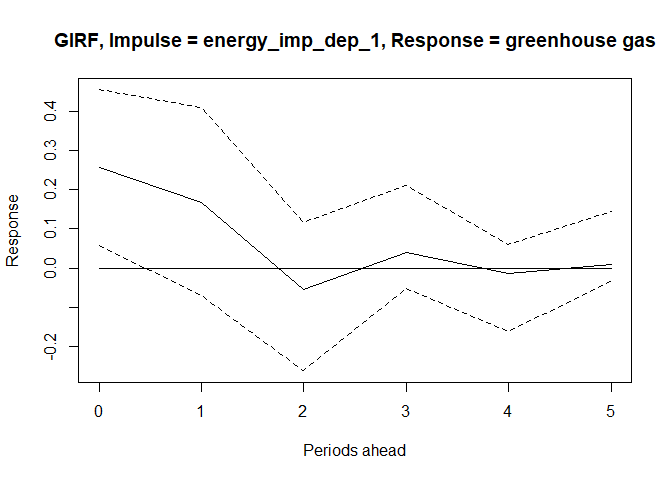
\includegraphics[width=0.7\textwidth]{images/IRF/IRF Analysis model 2-1.png}
    \caption{Forecasted GIRF, from energy imports dependency to greenhouse gases}
    \label{fig:IRF2_1}
\end{figure}

 \begin{figure}[H]
    \centering
    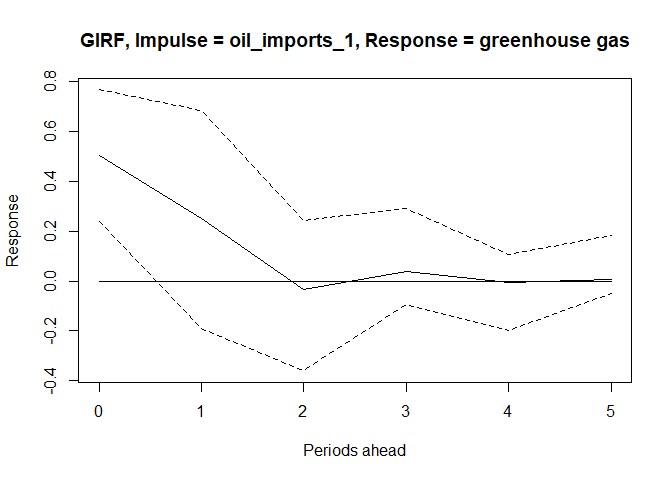
\includegraphics[width=0.7\textwidth]{images/IRF/IRF Analysis model 2-2.png}
    \caption{Forecasted GIRF, from oil imports to greenhouse gases}
    \label{fig:IRF2_2}
\end{figure}



\subsection*{Model 3} \label{Results_model3}
As in the previous paragraphs, table \ref{tab:tab_beta_3} shows the coefficients for both the frequentist and the bayesian estimation methods, while instead table \ref{tab:tab_sigma_3} reports the variance covariance matrix estimation in the case of a frequentist and bayesian approach. From table \ref{tab:tab_beta_3} bayesian approach showed overall smaller coefficients. Table \ref{tab:tab_sigma_3} shows instead that bayesian approach resulted in slightly higher values for the estimation of the variance while smaller estimation for the covariances.


\begin{table}[H]
\centering
\label{tab:tab_beta_3}
\begin{tabular}{|l|c|c|c|c|c|c|c|c|}
  \hline
 \multirow{2}{*}{Model3 $\hat{\beta}$} & \multicolumn{2}{c|}{$greenhouse_{t-1}$} & \multicolumn{2}{c|}{$GDP_{t-1}$}  & \multicolumn{2}{c|}{$fertilizer_{t-1}$} & \multicolumn{2}{c|}{$const$} \\  \cline{2-9}
 & $\hat{\beta}_{ols}$ & $\hat{\beta}_{B}$ & $\hat{\beta}_{ols}$ & $\hat{\beta}_{B}$ & $\hat{\beta}_{ols}$ & $\hat{\beta}_{B}$ & $\hat{\beta}_{ols}$ & $\hat{\beta}_{B}$\\
  \hline
    $greenhouse_{t}$ & -0.25 & -0.18 & 0.39 & 0.33 & 0.10  &  0.10 &  -0.13  & -0.12 \\ 
    $GDP_{t}$ & 0.17 & 0.19 & 0.17 &  0.14 & 0.01 & 0.01 & 0.03 & 0.03\\ 
    $fertilizer_{t}$ & -0.52 & -0.35 & -0.29 & 0.17 & 0.35 & 0.31 & -0.11 & -0.09 \\ 
   \hline
\end{tabular}
\caption{Bayesian and OLS estimation of $\hat{\beta}$, Model 3} \label{tab:tab_beta_3}
\end{table}

\begin{table}[H]
\centering
\begin{tabular}{|l|c|c|c|c|c|c|c|c|}
  \hline
 \multirow{2}{*}{Model 3 $\hat{\Sigma}$} & \multicolumn{2}{c|}{$greenhouse_{t-1}$} & \multicolumn{2}{c|}{$GDP_{t-1}$} & \multicolumn{2}{c|}{$fertilizer_{t-1}$} \\  \cline{2-7}
 & $\hat{\Sigma}_{ols}$ & $\hat{\Sigma}_{B}$ & $\hat{\Sigma}_{ols}$ & $\hat{\Sigma}_{B}$ & $\hat{\Sigma}_{ols}$ & $\hat{\Sigma}_{B}$ \\
  \hline
    $greenhouse_{t-1}$ & 0.09 & 0.12 & 0.09 & 0.08 & 0.07  &  0.06   \\ 
    $GDP_{t-1}$ & 0.09 & 0.08 & 0.20 &  0.22 & 0.06 & 0.05 \\ 
    $fertilizer_{t-1}$ & 0.07 & 0.06 & 0.06 & 0.05 & 0.32 & 0.33 \\ 
   \hline
\end{tabular}
\caption{Bayesian and OLS estimation of $\hat{\Sigma}$, Model 3} \label{tab:tab_sigma_3}
\end{table}
\\


From the forecasted GIRF depicted in the following figures \ref{fig:IRF3_1} and \ref{fig:IRF3_2} we can say that even if the one standard deviation increase in GDP per capita has a higher response and tents to decrease less steeper with respect to the same shock given the kg/ha fertilizers, they both cause the same increasing effect to greenhouse gases. In the end we can conclude that both GDP per capita and fertilizers does contribute to the release of greenhouse gases into the atmosphere.

 \begin{figure}[H]
    \centering
    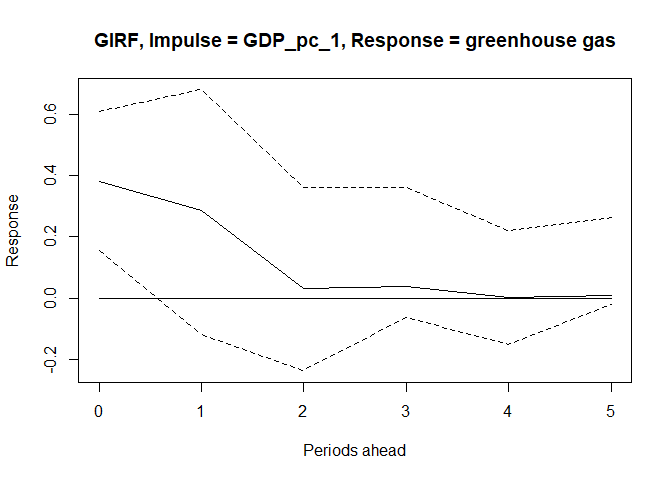
\includegraphics[width=0.7\textwidth]{images/IRF/IRF Analysis model 3-1.png}
    \caption{Forecasted GIRF, from GDP pc to greenhouse gases}
    \label{fig:IRF3_1}
\end{figure}

 \begin{figure}[H]
    \centering
    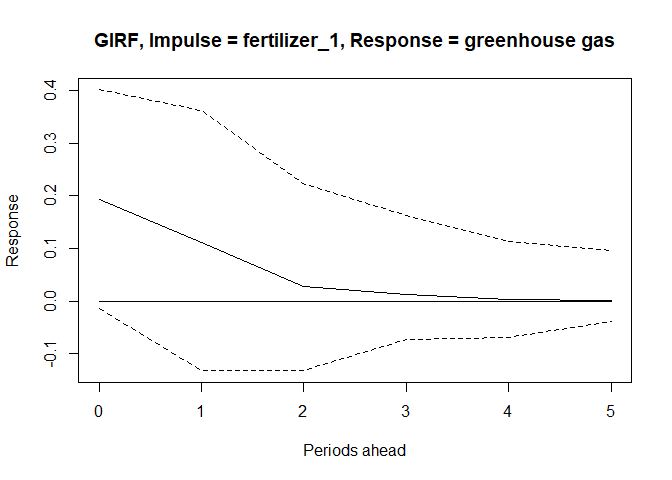
\includegraphics[width=0.7\textwidth]{images/IRF/IRF Analysis model 3-2.png}
    \caption{Forecasted GIRF, from fertilizer to greenhouse gases}
    \label{fig:IRF3_2}
\end{figure}


\clearpage

\section{Conclusions and suggested improvements} \label{Conclusions}
This analysis we had the objective of finding factors that contributed to the amount of greenhouse emission and measure their impact. For this purpose we collected yearly data of potential causes ranging from 1990 to 2020 for Italy.\\

We modeled the data using VAR models, which coefficient were estimated with bayesian methods and MCMC sampling. We also computed the forecast of the GIRF to measure the relations between variables. Our main conclusions are stated as follows:\\

\begin{itemize}
    \item We obtained practically the same coefficients of the OLS estimation using bayesian methods, although the estimated variance covariance matrices were different from OLS, specifically the variances were higher in the bayesian framework while the covariances were higher in the OLS.
    \item Our first model included Harvested rice and land under permanent crops as variables. They both seem to contribute positively and with the same magnitude to the increase of greenhouse gas emissions. The shocks fade away after the second year.
    \item The second model was characterised by energy imports dependency and oil imports. Both showed similar patterns when estimating the GIRF, contributing positively to the greenhouse gasses emissions. The shocks seems to fade around the fourth year. 
    \item The last model included GDP per capita and kg/ha of fertilizers. GDP per capita showed a higher impact to greenhouse gases with respect to the one caused by fertilizers. This could be a sign of how economic growth is leveraged on emissions of this type.
    \item According to the research we did upfront and our prior knowledge on the topic, the impact from agriculture, the economy and fossil fuels were as expected. Improvements in the modeling phase could lead to more precise measurements of the effects. 
    \item Further improvements could come from the use of a longer and more frequent (monthly or quarterly data) time series, modeling greenhouse gases components separately and more complex models.
\end{itemize}

\clearpage

\begin{center}
    \section{Bibliography}
\end{center}
\printbibliography
\clearpage


\section{Appendix} \label{Appendix}
\subsection{Model 1: Chain analysis}

\begin{figure}[!htb]
   \begin{minipage}{0.48\textwidth}
     \centering
     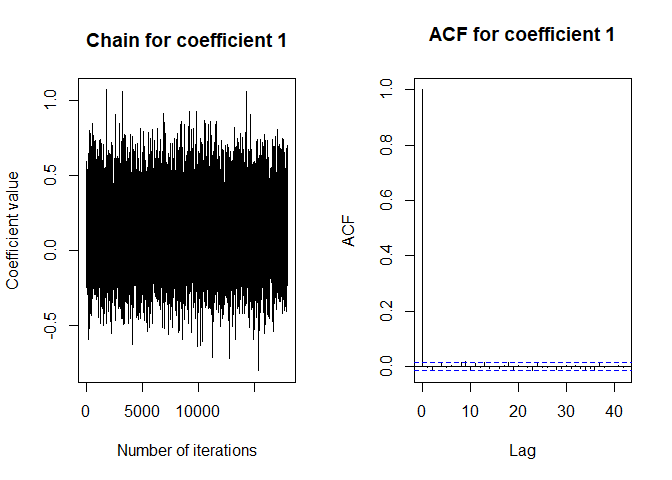
\includegraphics[width=1\linewidth]{images/Chain traces_1/Chain analysis model 1-1.png}
     \caption{Chain 1}\label{Fig:Chain 1}
   \end{minipage}\hfill
   \begin{minipage}{0.48\textwidth}
     \centering
     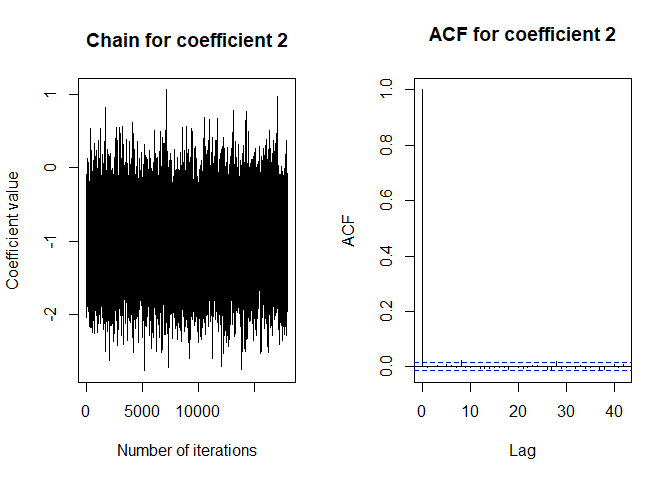
\includegraphics[width=1\linewidth]{images/Chain traces_1/Chain analysis model 1-2.png}
     \caption{Chain 2}\label{Fig: Chain 2}
   \end{minipage}
\end{figure}

\begin{figure}[!htb]
   \begin{minipage}{0.48\textwidth}
     \centering
     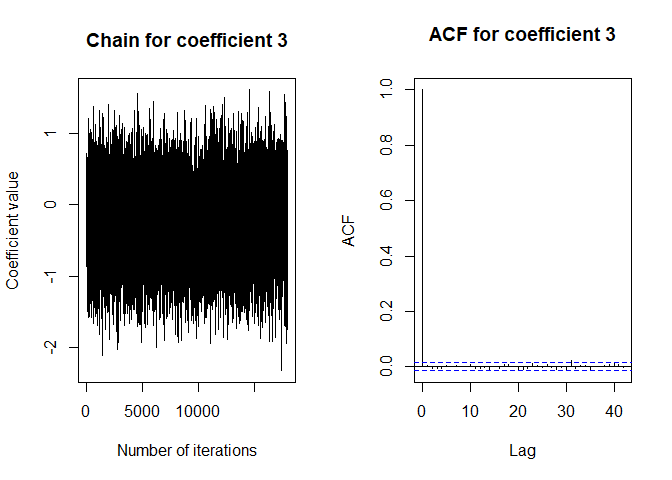
\includegraphics[width=1\linewidth]{images/Chain traces_1/Chain analysis model 1-3.png}
     \caption{Chain 3}\label{Fig:Chain 3}
   \end{minipage}\hfill
   \begin{minipage}{0.48\textwidth}
     \centering
     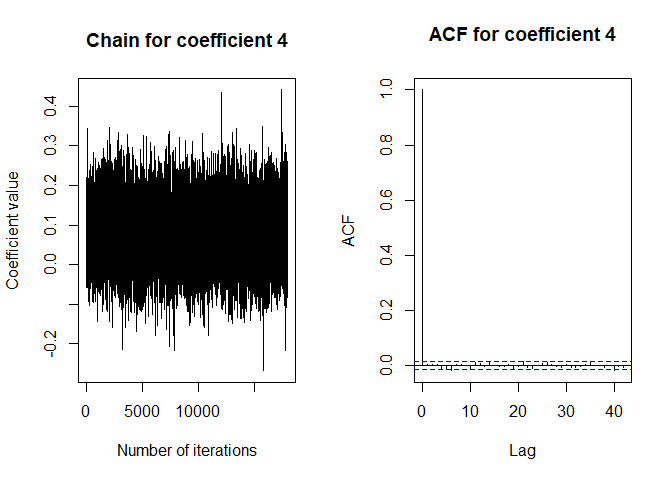
\includegraphics[width=1\linewidth]{images/Chain traces_1/Chain analysis model 1-4.png}
     \caption{Chain 4}\label{Fig: Chain 4}
   \end{minipage}
\end{figure}

\begin{figure}[!htb]
   \begin{minipage}{0.48\textwidth}
     \centering
     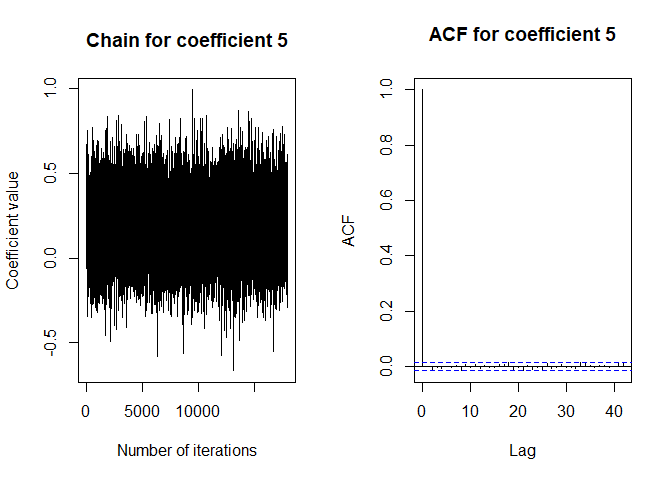
\includegraphics[width=1\linewidth]{images/Chain traces_1/Chain analysis model 1-5.png}
     \caption{Chain 5}\label{Fig:Chain 5}
   \end{minipage}\hfill
   \begin{minipage}{0.48\textwidth}
     \centering
     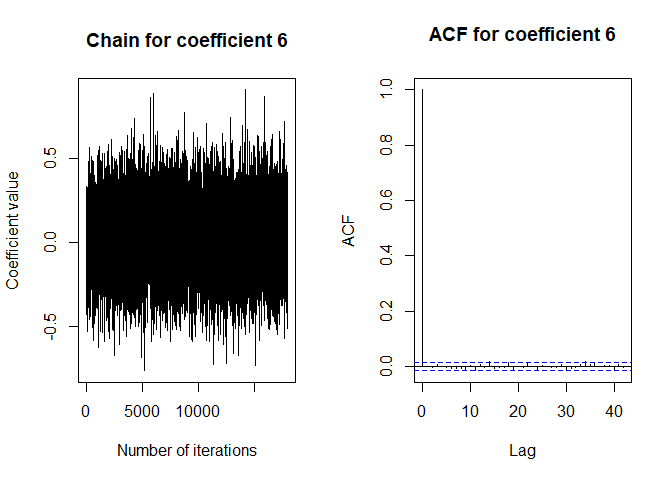
\includegraphics[width=1\linewidth]{images/Chain traces_1/Chain analysis model 1-6.png}
     \caption{Chain 6}\label{Fig: Chain 6}
   \end{minipage}
\end{figure}

\begin{figure}[!htb]
   \begin{minipage}{0.48\textwidth}
     \centering
     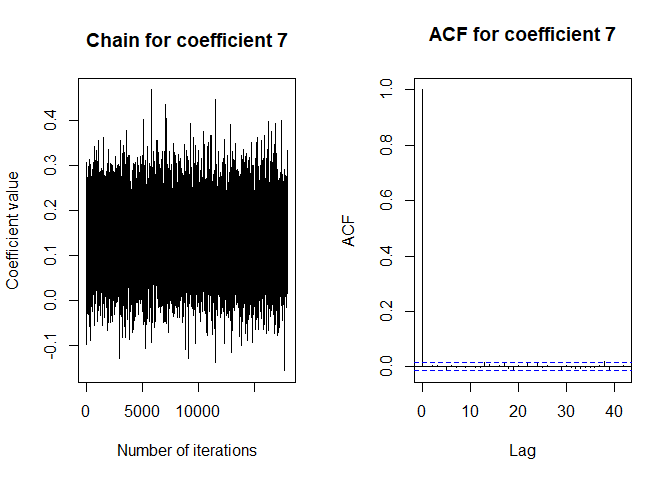
\includegraphics[width=1\linewidth]{images/Chain traces_1/Chain analysis model 1-7.png}
     \caption{Chain 7}\label{Fig:Chain 7}
   \end{minipage}\hfill
   \begin{minipage}{0.48\textwidth}
     \centering
     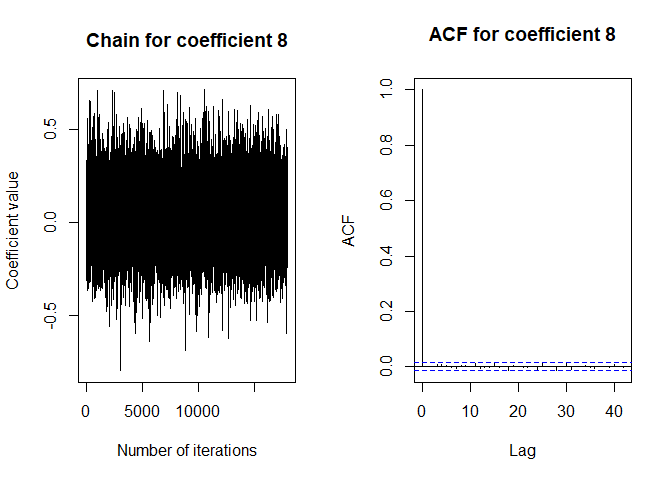
\includegraphics[width=1\linewidth]{images/Chain traces_1/Chain analysis model 1-8.png}
     \caption{Chain 8}\label{Fig: Chain 8}
   \end{minipage}
\end{figure}

\begin{figure}[!htb]
   \begin{minipage}{0.48\textwidth}
     \centering
     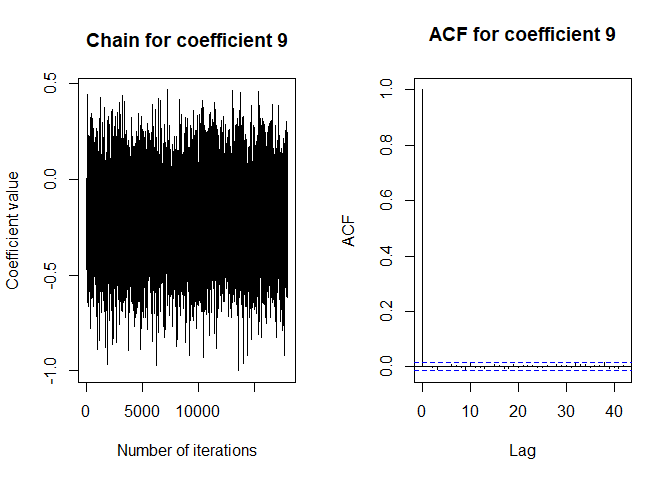
\includegraphics[width=1\linewidth]{images/Chain traces_1/Chain analysis model 1-9.png}
     \caption{Chain 9}\label{Fig:Chain 9}
   \end{minipage}\hfill
   \begin{minipage}{0.48\textwidth}
     \centering
     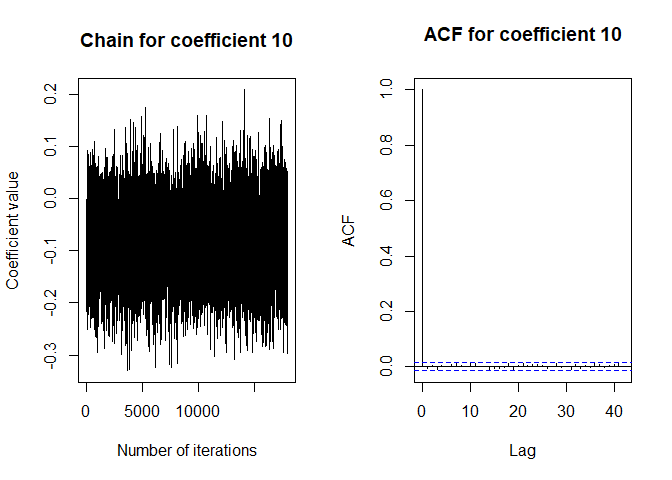
\includegraphics[width=1\linewidth]{images/Chain traces_1/Chain analysis model 1-10.png}
     \caption{Chain 10}\label{Fig: Chain 10}
   \end{minipage}
\end{figure}

\begin{figure}[!htb]
   \begin{minipage}{0.48\textwidth}
     \centering
     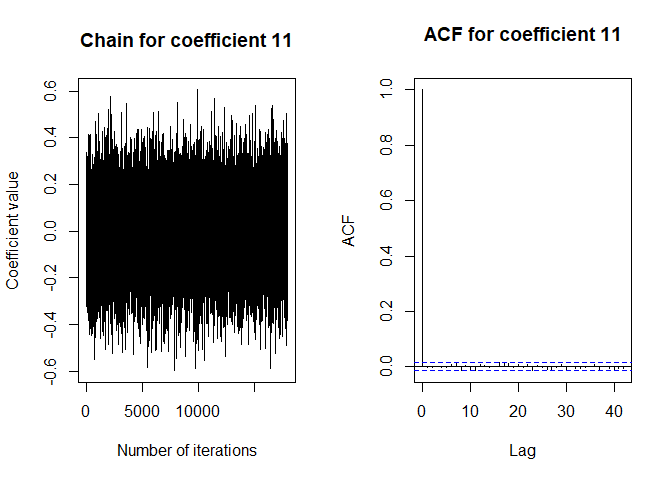
\includegraphics[width=1\linewidth]{images/Chain traces_1/Chain analysis model 1-11.png}
     \caption{Chain 11}\label{Fig:Chain 11}
   \end{minipage}\hfill
   \begin{minipage}{0.48\textwidth}
     \centering
     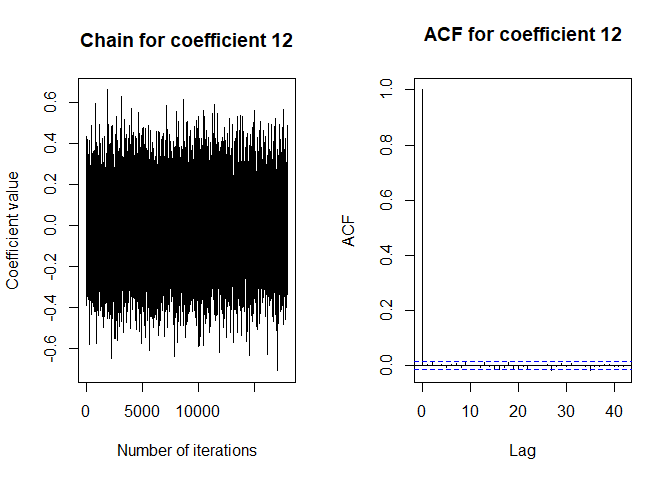
\includegraphics[width=1\linewidth]{images/Chain traces_1/Chain analysis model 1-12.png}
     \caption{Chain 12}\label{Fig: Chain 12}
   \end{minipage}
\end{figure}


 \begin{figure}[h]
    \centering
    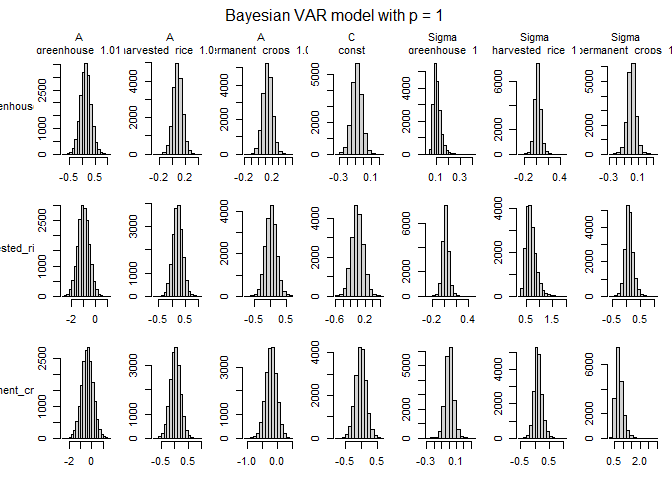
\includegraphics[width=1\textwidth]{images/Chains densities/Chain analysis model 1-13.png}
    \caption{Chain densities}
    \label{fig:Chain densities}
\end{figure}

\clearpage
\subsection{Model 2: Chain analysis}

\begin{figure}[!htb]
   \begin{minipage}{0.48\textwidth}
     \centering
     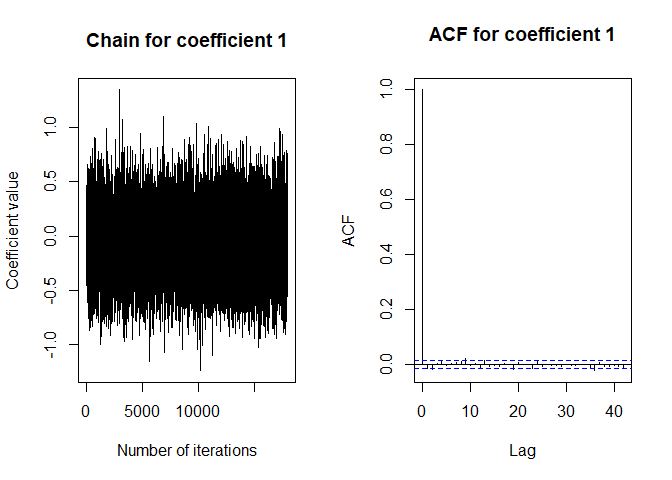
\includegraphics[width=1\linewidth]{images/Chain traces_2/Chain analysis model 2-1.png}
     \caption{Chain 1}\label{Fig:Chain 1}
   \end{minipage}\hfill
   \begin{minipage}{0.48\textwidth}
     \centering
     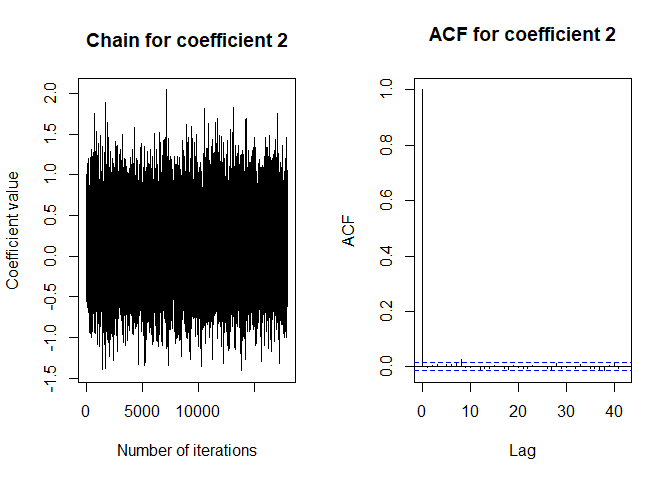
\includegraphics[width=1\linewidth]{images/Chain traces_2/Chain analysis model 2-2.png}
     \caption{Chain 2}\label{Fig: Chain 2}
   \end{minipage}
\end{figure}

\begin{figure}[!htb]
   \begin{minipage}{0.48\textwidth}
     \centering
     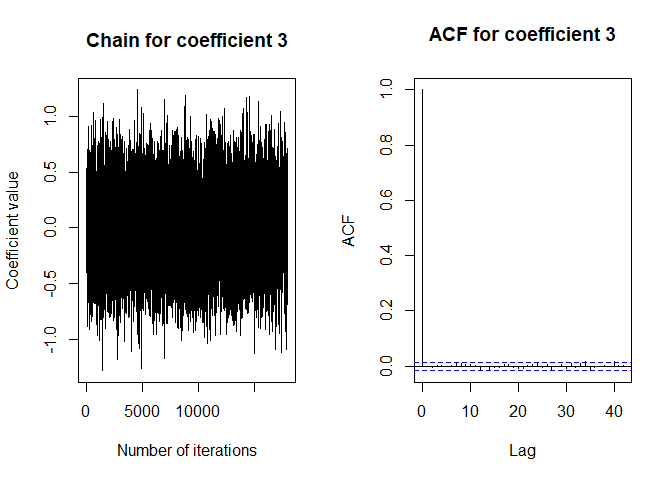
\includegraphics[width=1\linewidth]{images/Chain traces_2/Chain analysis model 2-3.png}
     \caption{Chain 3}\label{Fig:Chain 3}
   \end{minipage}\hfill
   \begin{minipage}{0.48\textwidth}
     \centering
     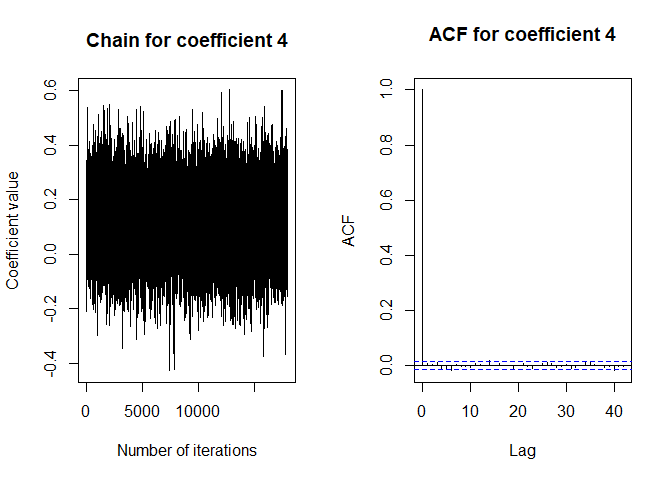
\includegraphics[width=1\linewidth]{images/Chain traces_2/Chain analysis model 2-4.png}
     \caption{Chain 4}\label{Fig: Chain 4}
   \end{minipage}
\end{figure}

\begin{figure}[!htb]
   \begin{minipage}{0.48\textwidth}
     \centering
     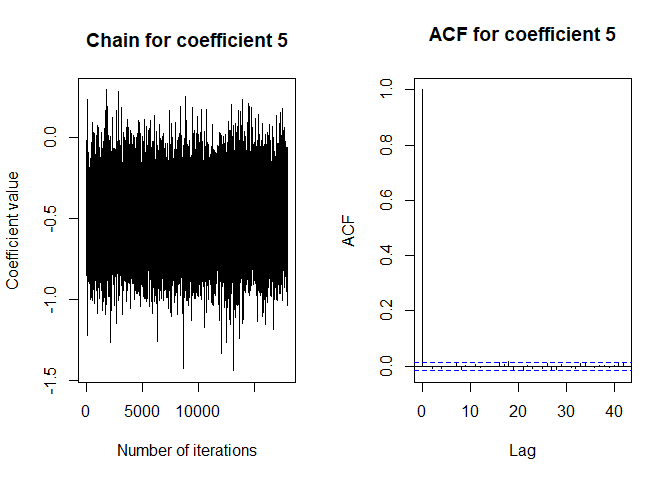
\includegraphics[width=1\linewidth]{images/Chain traces_2/Chain analysis model 2-5.png}
     \caption{Chain 5}\label{Fig:Chain 5}
   \end{minipage}\hfill
   \begin{minipage}{0.48\textwidth}
     \centering
     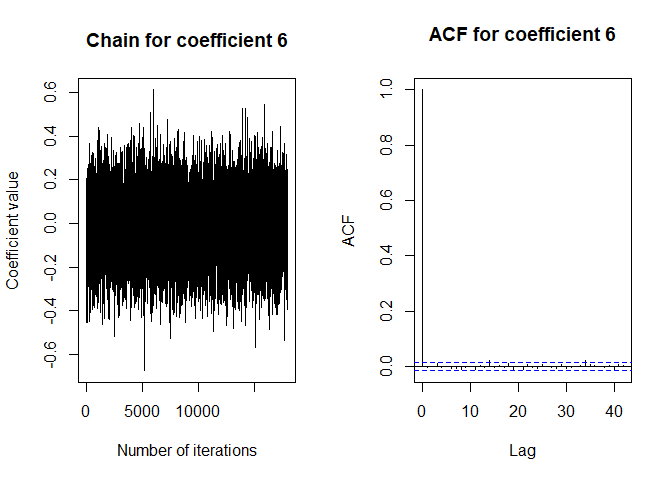
\includegraphics[width=1\linewidth]{images/Chain traces_2/Chain analysis model 2-6.png}
     \caption{Chain 6}\label{Fig: Chain 6}
   \end{minipage}
\end{figure}

\begin{figure}[!htb]
   \begin{minipage}{0.48\textwidth}
     \centering
     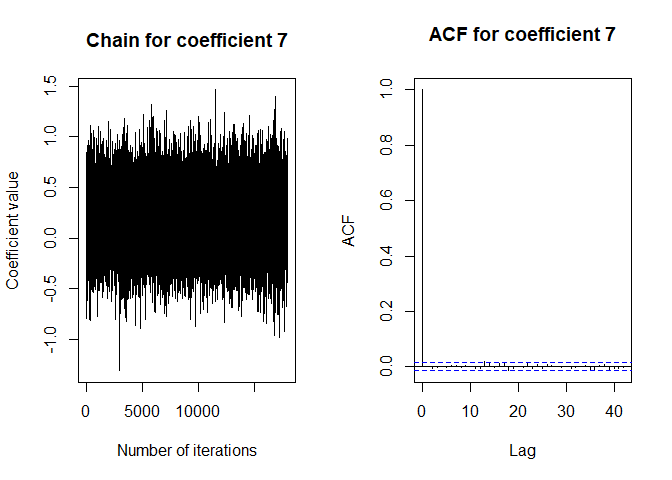
\includegraphics[width=1\linewidth]{images/Chain traces_2/Chain analysis model 2-7.png}
     \caption{Chain 7}\label{Fig:Chain 7}
   \end{minipage}\hfill
   \begin{minipage}{0.48\textwidth}
     \centering
     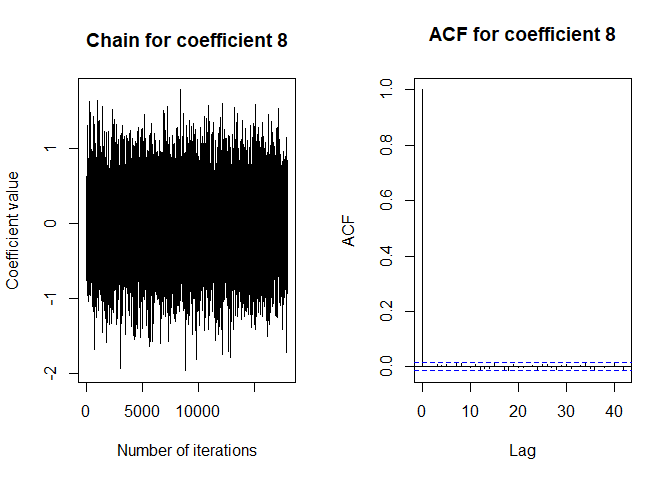
\includegraphics[width=1\linewidth]{images/Chain traces_2/Chain analysis model 2-8.png}
     \caption{Chain 8}\label{Fig: Chain 8}
   \end{minipage}
\end{figure}

\begin{figure}[!htb]
   \begin{minipage}{0.48\textwidth}
     \centering
     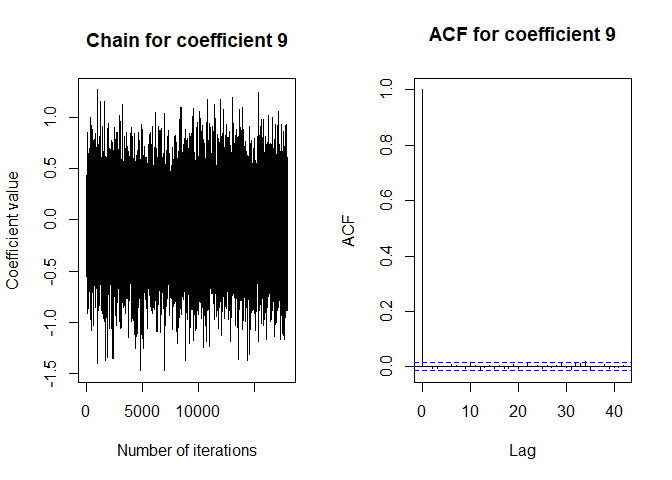
\includegraphics[width=1\linewidth]{images/Chain traces_2/Chain analysis model 2-9.png}
     \caption{Chain 9}\label{Fig:Chain 9}
   \end{minipage}\hfill
   \begin{minipage}{0.48\textwidth}
     \centering
     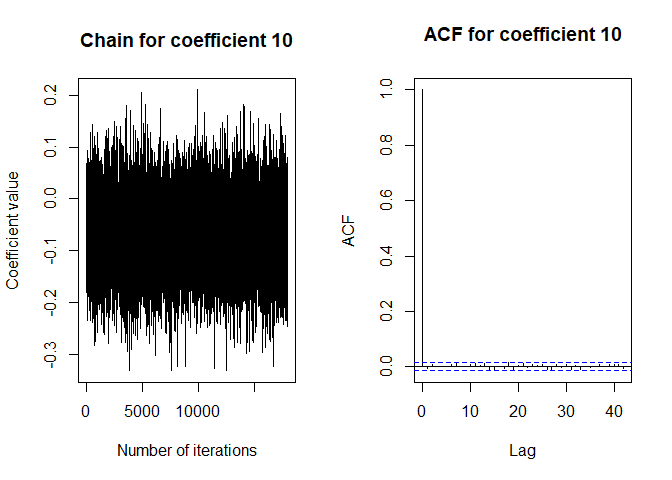
\includegraphics[width=1\linewidth]{images/Chain traces_2/Chain analysis model 2-10.png}
     \caption{Chain 10}\label{Fig: Chain 10}
   \end{minipage}
\end{figure}

\begin{figure}[!htb]
   \begin{minipage}{0.48\textwidth}
     \centering
     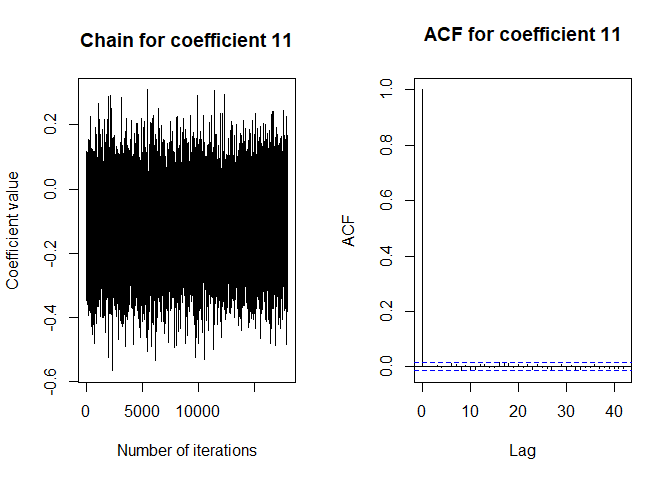
\includegraphics[width=1\linewidth]{images/Chain traces_2/Chain analysis model 2-11.png}
     \caption{Chain 11}\label{Fig:Chain 11}
   \end{minipage}\hfill
   \begin{minipage}{0.48\textwidth}
     \centering
     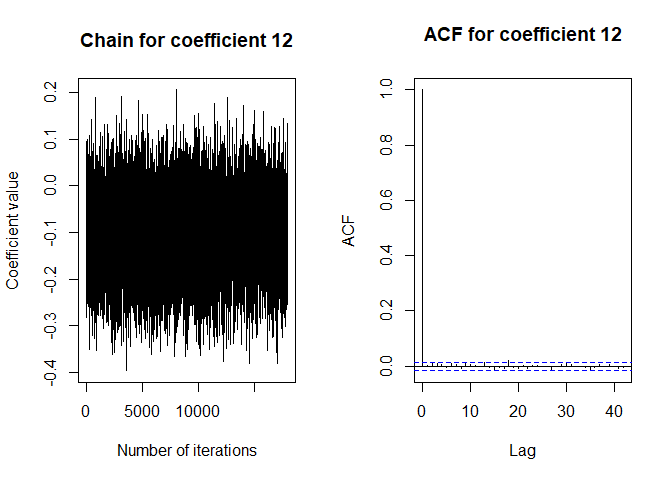
\includegraphics[width=1\linewidth]{images/Chain traces_2/Chain analysis model 2-12.png}
     \caption{Chain 12}\label{Fig: Chain 12}
   \end{minipage}
\end{figure}


 \begin{figure}[h]
    \centering
    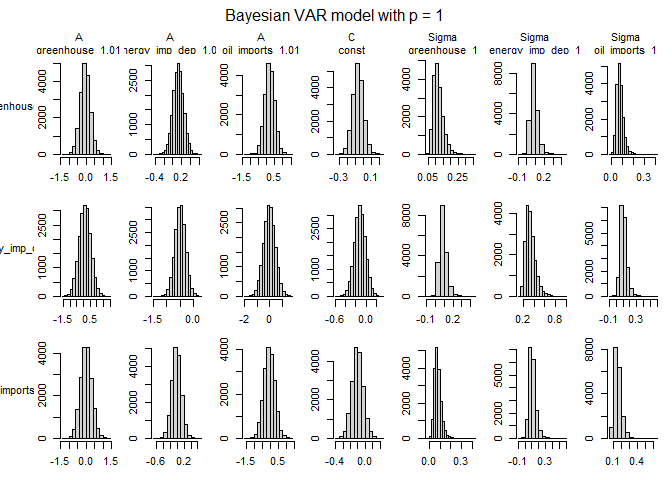
\includegraphics[width=1\textwidth]{images/Chains densities/Chain analysis model 2-13.png}
    \caption{Chain densities}
    \label{fig:Model 2: Chain densities}
\end{figure}

\clearpage
\subsection{Model 3: Chain analysis}

\begin{figure}[!htb]
   \begin{minipage}{0.48\textwidth}
     \centering
     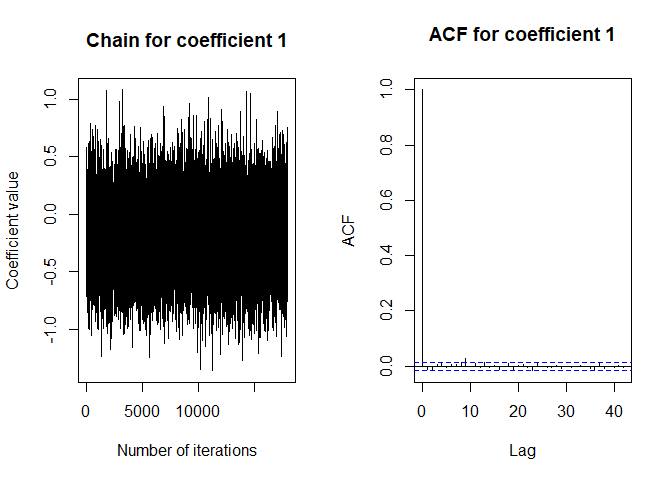
\includegraphics[width=1\linewidth]{images/Chain traces_3/Chain analysis-1.png}
     \caption{Chain 1}\label{Fig:Chain 1}
   \end{minipage}\hfill
   \begin{minipage}{0.48\textwidth}
     \centering
     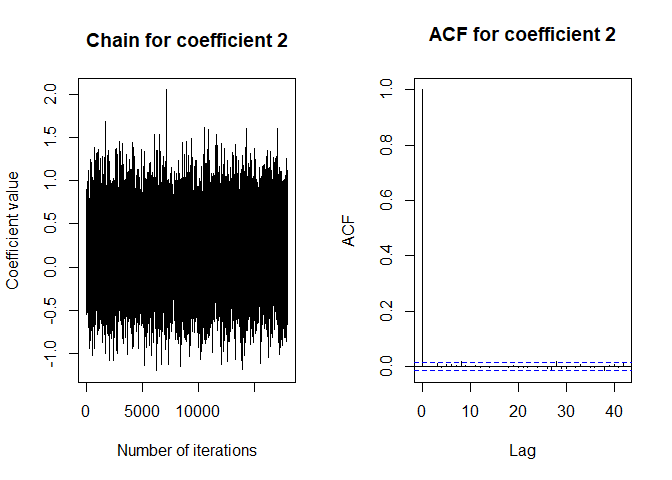
\includegraphics[width=1\linewidth]{images/Chain traces_3/Chain analysis-2.png}
     \caption{Chain 2}\label{Fig: Chain 2}
   \end{minipage}
\end{figure}

\begin{figure}[!htb]
   \begin{minipage}{0.48\textwidth}
     \centering
     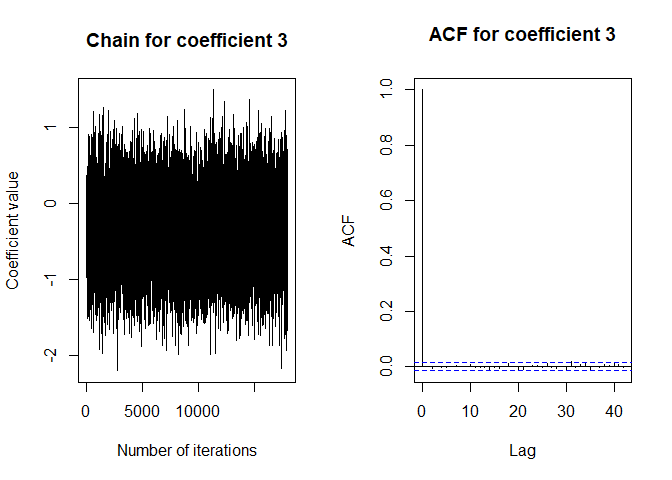
\includegraphics[width=1\linewidth]{images/Chain traces_3/Chain analysis-3.png}
     \caption{Chain 3}\label{Fig:Chain 3}
   \end{minipage}\hfill
   \begin{minipage}{0.48\textwidth}
     \centering
     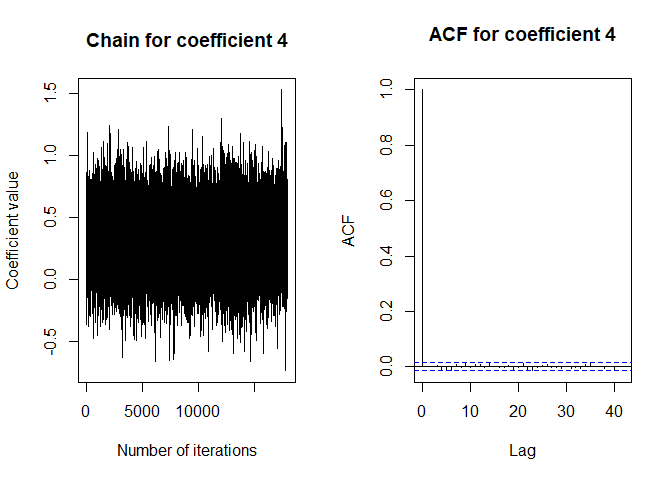
\includegraphics[width=1\linewidth]{images/Chain traces_3/Chain analysis-4.png}
     \caption{Chain 4}\label{Fig: Chain 4}
   \end{minipage}
\end{figure}

\begin{figure}[!htb]
   \begin{minipage}{0.48\textwidth}
     \centering
     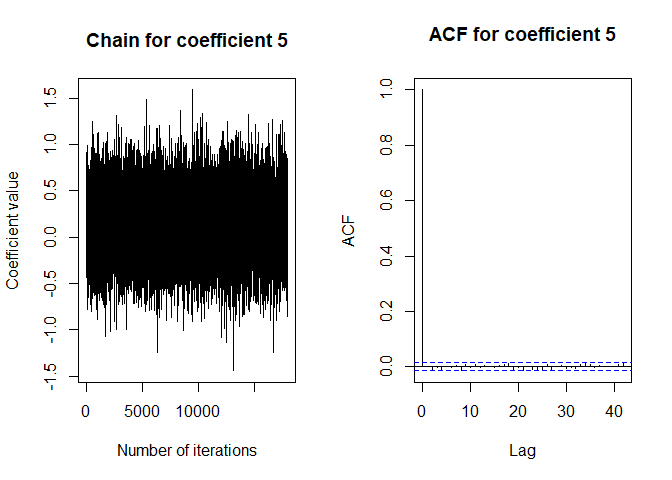
\includegraphics[width=1\linewidth]{images/Chain traces_3/Chain analysis-5.png}
     \caption{Chain 5}\label{Fig:Chain 5}
   \end{minipage}\hfill
   \begin{minipage}{0.48\textwidth}
     \centering
     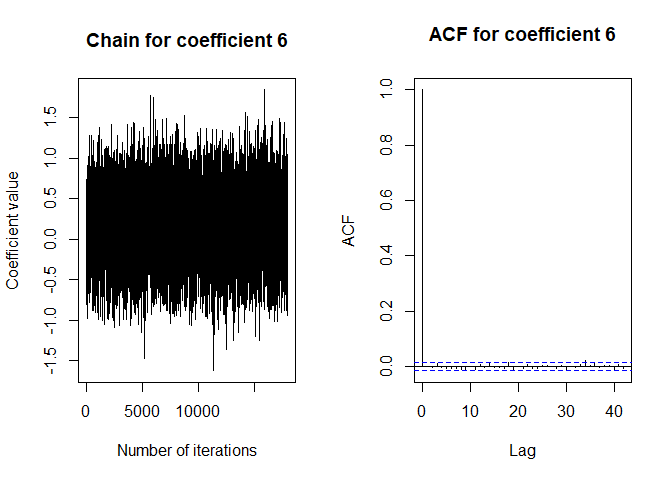
\includegraphics[width=1\linewidth]{images/Chain traces_3/Chain analysis-6.png}
     \caption{Chain 6}\label{Fig: Chain 6}
   \end{minipage}
\end{figure}

\begin{figure}[!htb]
   \begin{minipage}{0.48\textwidth}
     \centering
     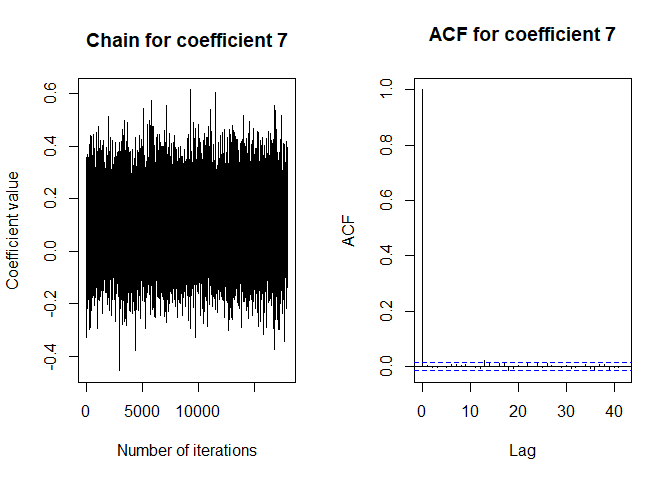
\includegraphics[width=1\linewidth]{images/Chain traces_3/Chain analysis-7.png}
     \caption{Chain 7}\label{Fig:Chain 7}
   \end{minipage}\hfill
   \begin{minipage}{0.48\textwidth}
     \centering
     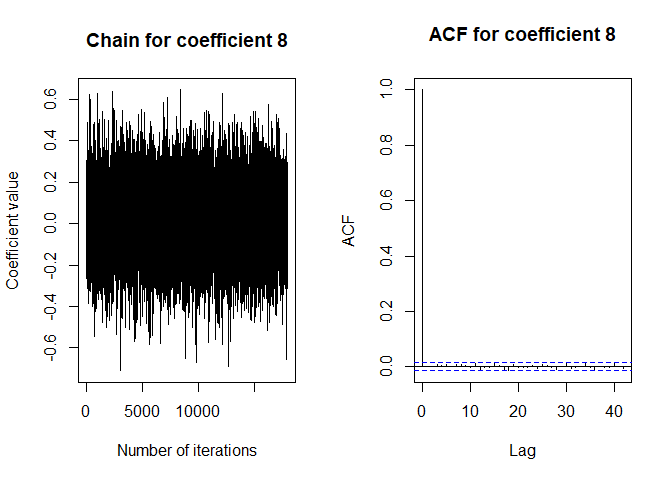
\includegraphics[width=1\linewidth]{images/Chain traces_3/Chain analysis-8.png}
     \caption{Chain 8}\label{Fig: Chain 8}
   \end{minipage}
\end{figure}

\begin{figure}[!htb]
   \begin{minipage}{0.48\textwidth}
     \centering
     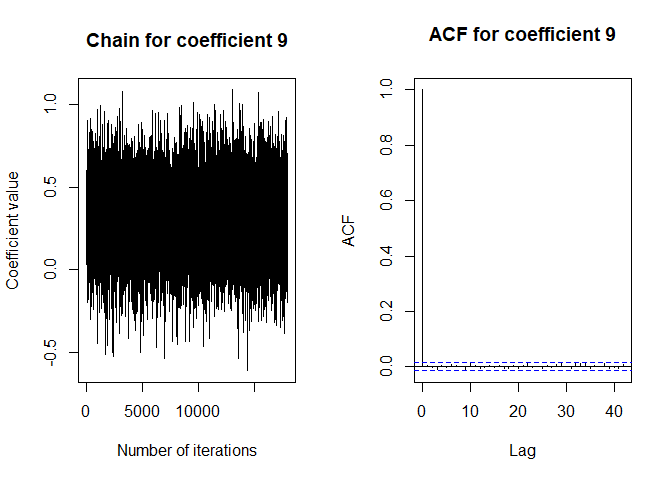
\includegraphics[width=1\linewidth]{images/Chain traces_3/Chain analysis-9.png}
     \caption{Chain 9}\label{Fig:Chain 9}
   \end{minipage}\hfill
   \begin{minipage}{0.48\textwidth}
     \centering
     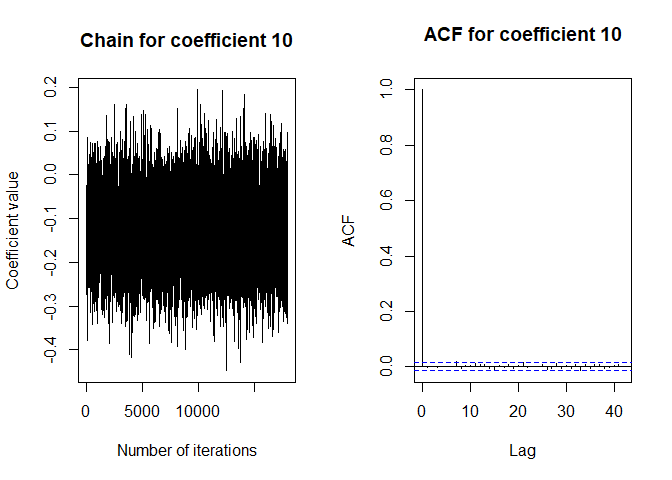
\includegraphics[width=1\linewidth]{images/Chain traces_3/Chain analysis-10.png}
     \caption{Chain 10}\label{Fig: Chain 10}
   \end{minipage}
\end{figure}

\begin{figure}[!htb]
   \begin{minipage}{0.48\textwidth}
     \centering
     \includegraphics[width=1\linewidth]{images/Chain traces_3/Chain analysis-11.png}
     \caption{Chain 11}\label{Fig:Chain 11}
   \end{minipage}\hfill
   \begin{minipage}{0.48\textwidth}
     \centering
     \includegraphics[width=1\linewidth]{images/Chain traces_3/Chain analysis-12.png}
     \caption{Chain 12}\label{Fig: Chain 12}
   \end{minipage}
\end{figure}


 \begin{figure}[h]
    \centering
    \includegraphics[width=1\textwidth]{images/Chains densities/Chain analysis-13.png}
    \caption{Chain densities}
    \label{fig:Model 3: Chain densities}
\end{figure}

\\



\end{document}